%\paragraph*{Nominal sets}

We start by briefly introducing the nominal sets framework, which will be the basis of much of this paper. Intuitively, nominal sets are sets where names are baked in from the outset.

Let us fix $\Atoms$ to be a countably infinite set of \boldemph{names} (or \boldemph{data values}) upon which nominal sets are built. 
    A permutation $\pi$ on $\Atoms$ (i.e.\ a bijection $\pi:\Atoms\to\Atoms$) is considered \emph{finite} if $\supp(\pi) = \{a \in \Atoms\mid \pi(a) \neq a\}$ is finite.
 For example, the identity permutation $id$ is finite ($id(a)=a$ for all $a\in\Atoms$) and, for any $a,b\in\Atoms$, so is the permutation $\swp{a}{b}$ given by:\ 
%     \[
%       \swp{a_1}{a_2}(x) =\begin{cases}
% a_{3-i} & \text{ if }x=a_i \\ x & \text{ if }x\neq a_1,a_2
%                          \end{cases}
%                        \]
$\swp{a}{b}(a) = b$, $\swp{a}{b}(b) = a$, and $\swp{a}{b}(x) = x$ for all $x\neq a,b$.  
 We denote the set of all finite permutations in $\Atoms$ as $\Perm$.
                       
\begin{definition}[\cite{PittsGabbay,Pitts}]\label{def:nomset}
    A \boldemph{nominal set} $\Xcal$ is a set $X$ equipped with an action from $\Perm$, i.e.\ a function $\_ \cdot \_: \Perm \times X \rightarrow X$ such that for all $x \in X$ and  $\pi, \pi' \in \Perm$:
    \[
    \pi \cdot (\pi' \cdot x) = (\pi \circ \pi') \cdot x,\ id \cdot x = x
    \]
    A set of names $\S\subseteq \Atoms$ \emph{supports} an element $x \in X$ if, for all $\pi \in \Perm$, if $\pi$ fixes all elements of $\S$ then $\pi\cdot x=x$. We stipulate that all elements of $X$ be \emph{finitely supported}, i.e.\ for all $x\in X$ there is some finite $\S\subseteq\Atoms$ that supports $x$. We write $\supp(x)$ for \emph{the support of $x$}, i.e.\ the least set supporting $x$. We say that $a$ \emph{is fresh for $x$}, and write $a\# x$, if $a\notin\supp(x)$.
\end{definition}

By abuse of notation, we may identify $\Xcal$ with its carrier set $X$. 
The action on a nominal set extends to products and subsets by $\pi \cdot(x,y) = (\pi \cdot x, \pi \cdot y)$ and, for any $S \subseteq \Xcal$, by $\pi \cdot S = \{\pi \cdot x \mid x \in S\}$. 
Additionally, if $\Xcal, \Ycal$ are nominal sets then so is $\Xcal \times \Ycal$, and the set of subsets of $\Xcal$ with finite support.
Accordingly, given a relation $R\subseteq\Xcal\times\Ycal$ and $\pi\in\Perm$, we have $\pi\cdot R=\{(\pi\cdot x,\pi\cdot y)\mid (x,y)\in R\}$. We call $R$ \emph{equivariant} if $\supp(R)=\emptyset$, i.e.\ for all $\pi$ and $(x,y)\in\Xcal\times\Ycal$, $(x,y)\in R\iff (\pi\cdot x,\pi\cdot y)\in R$. 

A notion in nominal sets we will be making extensive use of is that of an \emph{orbit}.

\begin{definition}
    Let $\Xcal$ be a nominal set. 
    Two elements $x, y\in \Xcal$ are \emph{nominally equivalent} (denoted $x \nomeq y$) if $\pi \cdot x = y$ for some $\pi\in\Perm$. Note $\nomeq$ is an equivalence relation.
    \\
For each $x \in \Xcal$, we define its \boldemph{orbit} $\orbs(x)$ to be its $\nomeq$-equivalence class; whereas for each finite $\S\subseteq\Atoms$ we let $\orbs[\S](x)$ be its \boldemph{$\S$-orbit}, i.e.\ its closure under permutations fixing $\S$:
    \begin{align*}
        \orbs(x) &= \{\pi \cdot x \mid \pi \in \Perm\} &
    \orbs[\S](x) &= \{\pi \cdot x \mid \forall a\in\S.\,\pi(a)=a\}
    \end{align*}
    Observe that $\orbs(x)=\orbs[\emptyset](x)$.
    Moreover, for any $S\subseteq \Xcal$ with finite support we let:
    \begin{itemize}
    \item
the {\em closure} of $S$ be\
        $\cls{}(S) = \{\pi\cdot x\mid x\in S\land\pi\in\Perm\}$;
      \item the \emph{set of orbits} of $S$ be\
   $
        \orb(S) = \{ \orbs[\supp(S)](x) \mid x \in S\}
    $.
      \end{itemize}
We say that a nominal set $\Xcal$ is \boldemph{orbit-finite} if $\orb(\Xcal)$ is finite.
If $\Xcal$ is orbit-finite, we let its \emph{register index} be\
    $
        \regindex(\Xcal) = \max\{|\supp(x)| \mid x \in \Xcal\}
        $.\ntnote{can we find a standard term for this, e.g. from Pitts}
\end{definition}

Note in particular that
$\orbs(x)=\cls{}(\{x\})$, for any $x\in\Xcal$, and
$\orb(\Xcal) = \{ \orbs(x) \mid x \in \Xcal\}$.
Moreover, for any finitely supported $S\subseteq\Xcal$ we can see by inspection that:
\[\bigcup\orb(S)=S\subseteq\cls{}(S)\subseteq\Xcal
  \]
and $\supp(\cls{}(S))=\emptyset$. Some useful albeit more technical properties follow.

\begin{restatable}{lemma}{nomlemma}\label{lem:nomlemma}
	Let $\Xcal,\Ycal$ be nominal sets and $X,Y \subseteq \Xcal$. 
	Then:
	\begin{enumerate}
		\item\label{nomlemma:orbs} $\{\orbs(x) \mid x \in X\} = \orb(\cls{}(X))$ and $|\orb(\cls{}(X))| \le |\orb(X)|$;
		\item\label{nomlemma:cls} if $X$ has empty support then $\cls{}(X \times Y) = X \times \cls{}(Y)$;
		\item\label{nomlemma:prod} if $\Xcal,\Ycal$ are orbit-finite then
		$|\orb(\Xcal \times \Ycal)| \le |\orb(\Xcal)|\cdot|\orb(\Ycal)|\cdot {n_1}^{n_2}\cdot(1 + \epsilon)$ where $\{n_1,n_2\}=\{\regindex(\Xcal), \regindex(\Ycal)\}\neq\{0\}$ and $n_1\geq n_2$,
		and $\epsilon\leq 1$ is a constant that vanishes for $n_2\geq 4$. 
	\end{enumerate}
\end{restatable}
\vspace{1em}


Orbit-finiteness essentially captures the notion of a set being ``finite up to permutation'', and it is central in the development of automata over nominal sets~\cite{automatanominalsets}.

We are going to define transition systems which retain a possibly unbounded history component but are otherwise finite. For that purpose, orbit-finiteness needs to be relaxed to accommodate histories of unbounded size. One part of our solution is to use configurations comprising a state and a history, where only the set of states is orbit-finite. The other part is to stipulate that the names appearing only in the history component of a configuration are in between them indistinguishable. This can be captured by the following notion.

\begin{definition}
  Given a nominal set $\Xcal$ and $x\in\Xcal$, for each $\S'\subseteq\S\subseteq\Atoms$, we say that the pair \emph{$(\S',\S)$ freshly supports $x$} if, for all $\pi\in\Perm$:
  \[ (\forall a\in\S'.\,\pi(a)=a\land\pi\cdot (\S\setminus\S')=\S\setminus\S')
    \implies \pi\cdot x=x.
  \]
\end{definition}

This notion of support refines ordinary support and, to the best of our knowledge, is novel. In particular, if $x$ is freshly supported by $(\S',\S)$ then it is supported by $\S$. Moreover, $x$ is freshly supported by $(\S,\S)$ iff it is supported by $\S$.

% There is also a notion of least finite fresh support.

% \begin{lemma} Given a nominal set $\Xcal$, each 
%  $x\in\Xcal$ is freshly supported by $(\bigcap)$.
% \end{lemma}

We can now move to our labelled transition systems. These are going to be nominal LTSs~\cite{automatanominalsets} (i.e.\ with states and labels being nominal sets) where each state is paired with a \emph{history} that includes the names (in the support) of the state. The history is updated in each transition to include any names of the label of said transition. 

\begin{definition}
A \emph{Fresh Nominal Labelled-Transition System (FLTS)}
is a tuple $\mathcal{L}=\langle \mathcal{S},L,\rightarrow\rangle$, where:
\begin{itemize}
\item $\mathcal{S}$ is a nominal set of \emph{states}
and $L$ is a nominal set of \emph{actions},
\item    ${\rightarrow}\subseteq \CONF\times L\times\CONF$ is an equivariant \emph{transition relation},
  \item 
  where
 $\CONF=\{(s,H)\in\Scal\times\PPfn(\Atoms)\mid \supp(s)\subseteq H\}$ is the nominal set of \emph{configurations};
\end{itemize}
and such that, for all $(s,H) \in \CONF$:
 \begin{itemize}
     \item 
 $\{(\ell, (s', H'))\mid (s, H) \xrightarrow{\ell} (s', H')\}$ is freshly supported by $(\supp(s),H)$,
\item
for all $(s, H) \xrightarrow{\ell} (s', H')$,\
$\supp(s')\subseteq \supp(s)\cup \supp(\ell)$ and 
$H'=H\cup \supp(\ell)$.
 \end{itemize}
 $\mathcal{L}$ is called \emph{fresh-orbit-finite} if $\cal S$ and $L$ are orbit-finite.
\end{definition}

This scenario applies to a range of examples, such as name-carrying processes (e.g.\ in the $\pi$-calculus) and name-manipulating programs (e.g.\ Java programs with objects). At the automata level, a member formalism is that of \emph{fresh-register automata}~\cite{fra}, which are the baseline paradigm in our study. As we are interested in behavioural properties, rather than language acceptance, we disregard initial and final states. %Below, we let $r$ be a natural number and write $[1,r]$ for the set $\{1,\dots,r\}$.
The automata we define next operate on inputs $(t,a)\in\Sigma\times\Atoms$ where $t$ comes from a finite set of \emph{tags} and $a$ is a name.  

\begin{definition}\label{def:FRAs}
  An $r$-\boldemph{Fresh-Register Automaton ($r$-FRA)} is a tuple $\Acal=\langle Q,\mu,\Sigma,\delta\rangle$, where $r\in\mathbb{N}$ is the number of \emph{registers} in $\Acal$ and:
  \begin{itemize}
  \item $Q$ is a finite set of \emph{states}, and $\mu:Q\to\Pcal([1,r])$ an \emph{availability function};
  \item $\Sigma$ is a finite set of {tags}, and
 $\delta:Q\times\Sigma\times\{i,\Lfr{i},\Gfr{i}\mid 1\leq i\leq r\}\times Q$ is the transition relation;
    \end{itemize}
    subject to the following conditions:
    \begin{itemize}
    \item if $(q,t,i,q')\in\delta$ then $i\in\mu(q)$ and $\mu(q')\subseteq\mu(q)$;
    \item
      if $(q,t,\Lfr i,q')\in\delta$ or $(q,t,\Gfr i,q')\in\delta$ then $\mu(q')\subseteq\mu(q)\cup\{i\}$.
    \end{itemize}
    We shall write $q\xrightarrow{t,x}q'$ for $(q,t,x,q')\in\delta$.
  \end{definition}

  We can see that the labels appearing in FRA transitions are of the form $(t,x)$, where $t$ comes from a finite alphabet while $x$ is a variant of a register index $i$.
Assuming the automaton is at state $q$ and given $q\xrightarrow{t,x}q'$, 
depending on $x$ the automaton will perform one of the following actions before moving to state $q'$:
  \begin{itemize}
  \item $x=i$: read the input $(t,a)$, where $a$ is the name currently in register $i$\,---\,note here that $i$ needs to be available at $q$ (i.e.\ $i\in\mu(q)$);
  \item $x=\Lfr{i}$: read any input $(t,a)$ so long $a$ is not currently stored in any register (i.e.\ it is \emph{locally fresh}), and store $a$ in register $i$;
  \item $x=\Gfr{i}$: read any input $(t,a)$ so long $a$ is has not be seen before (i.e.\ it is \emph{globally fresh}), and store $a$ in register $i$.
  \end{itemize}
Formally, the semantics of an FRA can be given in terms of its derived FLTS.
The latter features states of the form $(q,\rho)$ where $q$ is a state and $\rho$ an assignment of values to available registers, i.e.\ the ones in $\mu(q)$.
It is good to bear in mind that $q$ has empty support.

\begin{definition}
  Given an $r$-FRA $\Acal=\langle Q,\mu,\Sigma,\delta\rangle$ we define its FLTS $\Gcal_\Acal=\langle \Scal_\Acal,\Sigma\times\Atoms,\to\rangle$ by setting (and writing configurations simply as $(q,\rho,H)$ instead of $((q,\rho),H)$):
  \begin{itemize}
    \item 
$ \Scal_\Acal = \{(q,\rho)\mid q\in Q\land \rho:\mu(q)\to\Atoms\text{ injective}\}
$;
\item
  $(q,\rho,H)\xrightarrow{t,a}(q',\rho',H')$ whenever there is $q\xrightarrow{t,x}q'$ such that, for some register $i$:
  \begin{itemize}
    \item 
$x=i$ and $a=\rho(i)$, while $\rho'=\rho$; or
\item
$x=\Lfr i$ and $a\notin\rng(\rho)$, while $\rho'=\rho[i\mapsto a]\upharpoonright\mu(q')$; or
\item
$x=\Gfr i$ and $a\notin H$, while $\rho'=\rho[i\mapsto a]\upharpoonright\mu(q')$;
\end{itemize}
where $\rho[i\mapsto a]$ is the update of $\rho$ mapping $i$ to $a$, and the operator $\upharpoonright$ performs domain restriction. In all cases, $H'=H\cup\{a\}$.
\end{itemize}
\end{definition}

It is not difficult to verify that $\Gcal_\Acal$ is indeed an FLTS. First, the sets $\Scal_\Acal$ and $\Sigma\times\Atoms$ are closed under permutation, hence they are nominal sets. The definition of the transition relation does not single out any specific names and is therefore equivariant. What is more important, the names appearing in the history but not in the registers of a configuration are indistinguishable to the automaton, and that makes the fresh-support condition true. Finally, in every transition, names in the final register assignment are sourced from those of the initial assignment and the label, and the history is correctly updated.

We conclude this section with some motivating examples. These include example of properties used in the literature and simple properties one may want to check in a verification scenario.

%A fresh path is a path where all names are distinct.

\begin{example}\label{example:freshPaths}
  Let us assume a unique tag, e.g.\ $\Sigma=\{\bullet\}$, which we suppress for brevity.  
  Consider the following properties (cf.~\cite{KlinHD}):
  \begin{align*}
    &\text{\em All paths, finite and infinite, contain pairwise distinct names.}&\tag{\textsc{\#All}}\\
    &\text{\em There is an infinite path where all names are distinct.}&\tag{\textsc{\#Path}}
\end{align*}
Thus, both properties specify paths of the forms\ $a_1 a_2 \dots a_n$\ or\ $a_1 a_2a_3 \dots$\
where, for each $a_i$, there is no $j < i$ such that $a_i = a_j$. Let us now examine the following basic FRAs.

\noindent
\begin{centering}
\begin{tikzpicture}
  \node[state,initial,minimum size=5mm]   (q0) {$q_0$};
  \node[minimum size=5mm]   (r0) [below=1mm of q0] {$\emptyset$};
  \path[->] (q0) edge [loop right] node [right] {$\Gfr{1}$} (q0);
\end{tikzpicture}
\begin{tikzpicture}
  \node[state,initial,minimum size=5mm]   (q0) {$q_0$};
  \node[minimum size=5mm]   (r0) [below=1mm of q0] {$\emptyset$};
  \node[state,minimum size=5mm]   (q1) [right of=q0] {$q_1$};
  \node[minimum size=5mm]   (r1) [below=1mm of q1] {$\{1\}$};
  \path[->] (q1) edge [loop right] node [right] {$\Lfr{1}$} (q1);
  \path[->] (q0) edge node [above] {$\Lfr{1}$} (q1);
\end{tikzpicture}
\begin{tikzpicture}
  \node[state,initial,minimum size=5mm]   (q0) {$q_0$};
  \node[minimum size=5mm]   (r0) [below=1mm of q0] {$\emptyset$};
  \node[state,minimum size=5mm]   (q1) [right of=q0] {$q_1$};
  \node[minimum size=5mm]   (r1) [below=1mm of q1] {$\{1\}$};
  \path[->] (q1) edge [loop right] node [right] {$\Gfr{1}$} (q1);
  \path[->] (q0) edge node [above] {$\Lfr{1}$} (q1);
\end{tikzpicture}
% \begin{tikzpicture}
%   \node[state,initial,minimum size=5mm]   (q0) {$q_0$};
%   \node[state,accepting,minimum size=5mm] (q1) [right of=q0] {$q_1$};
%   \node[state,minimum size=5mm] (q2) [right of=q1] {$q_2$};

%   \path[->] (q0) edge [loop above] node [above] {$a$} (q0);
%   \path[->] (q0) edge [loop below] node [below] {$b$} (q0);
%   \path[->] (q0) edge node [above] {$b$} (q1);
%   \path[->] (q1) edge node [above] {$a$} (q2);
% \end{tikzpicture}
\end{centering}
\noindent
The sets beneath each state indicate available registers. The first FRA will engage in paths which always have distinct names, so it satisfies both \textsc{\#All} and \textsc{\#Path}. In fact, all three FRAs, from all possible configurations, satisfy \textsc{\#Path} as the locally fresh transitions can be realised by names that are in fact globally fresh. Moreover:
\begin{itemize}
\item the second FRA fails \textsc{\#All} from both states: for any $H,\rho,a,b$ with $a\#\rho, b$ and $i=0,1$, $(q_i,\rho,H)\xrightarrow{a}(q_1,[1\mapsto a],H\cup\{a\})\xrightarrow{b}(q_1,[1\mapsto b],H\cup\{a,b\})\xrightarrow{a}(q_1,[1\mapsto a],H\cup\{a,b\})$;
\item the third FRA satisfies \textsc{\#All} everywhere: even if going from $q_0$ to $q_1$ may involve an old name (already in history), the remaining names are all going to be globally fresh.
\end{itemize}
\end{example}

\ntnote{\scriptsize maybe present properties as above, giving them a name. It would be good to also include a taint example with freshness. Not sure about having FRAs for them as they take some space. If we do include FRAs then better not do Taint}
\begin{example}\label{example:sessions}
Let us assume a set of tags $\Sigma = \{\mathsf{S}, \mathsf{U}, \mathsf{T}\}$ which stand for $\mathsf{start}$, $\mathsf{use}$ and $\mathsf{terminate}$ respectively.
Consider an application in which a new session is created each time the application is launched.
This session can be used an arbitrary number of times, and then the session is terminated once the application is closed. 
We declare the following property for this application:
\[\begin{aligned}
	&\text{\em There is an infinite path that repeatedly starts a fresh session, arbitrarily uses it}\\
	&\text{\em and then terminates it.}
\end{aligned}\tag{\textsc{\#SUT}}\]
Once the session is terminated, it cannot be resumed or reactivated, a new session must be created.
A path for this will look as follows:
\[
	\mathsf{S}(s_1)\ \mathsf{U}(s_1)^*\ \mathsf{T}(s_1)\ \mathsf{S}(s_2)\ \mathsf{U}(s_2)^*\ \mathsf{T}(s_2)\ \mathsf{S}(s_3)\ \dots 
\]
where, for each $s_i$, there is no $j < i$ such that $s_i = s_j$.
Let us now consider this basic FRA:

\begin{centering}
 \begin{tikzpicture}
 	\node[state,initial,minimum size=5mm]   (q0) {$q_0$};
 	\node[minimum size=5mm]   (r0) [below=1mm of q0] {$\emptyset$};
 	\node[state,minimum size=5mm]   (q1) [right of=q0] {$q_1$};
 	\node[minimum size=5mm]   (r1) [below=1mm of q1] {$\{1\}$};
 	\path[->] (q1) edge [loop right] node [right] {$\mathsf{U}, {1}$} (q1);
 	\path[->] (q0) edge node [above] {$\mathsf{S}, \Gfr{1}$} (q1);
 	\path[->] (q1) edge [bend left] node [below] {$\mathsf{T}, 1$} (q0);
 \end{tikzpicture}
\end{centering}

\noindent
The FRA satisfies the property $\textsc{\#SUT}$ from $q_0$: for any $H, s_1,s_2$ with $s_1,s_2\notin H$, $H'=H\cup\{s_1\}$ and $H'' = H' \cup \{s_2\}$:

\begin{centering}
	 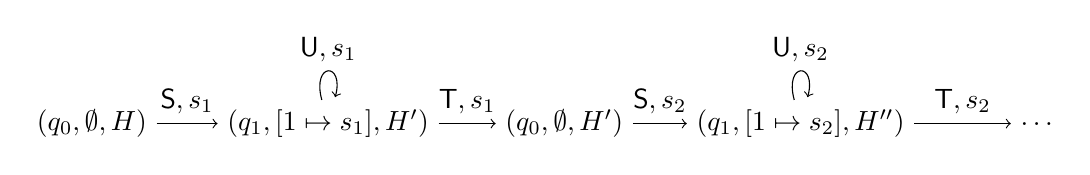
\begin{tikzpicture}[node distance=3cm]
		\node[minimum size=5mm]   (q0) {$(q_0, \emptyset, H)$};
		\node[minimum size=5mm]   (q1) [right of=q0] {$(q_1, [1\mapsto s_1], H')$};
		\node[minimum size=5mm]   (q2) [right of=q1] {$(q_0, \emptyset, H')$};
		\node[minimum size=5mm]   (q3) [right of=q2] {$(q_1, [1\mapsto s_2], H'')$};
		\node[minimum size=5mm]   (q4) [right of=q3] {$\dots$};
		\path[->] (q0) edge node [above] {$\mathsf{S}, s_1$} (q1);
		\path[->] (q1) edge [loop above] node [above] {$\mathsf{U}, s_1$} (q1);
		\path[->] (q1) edge node [above] {$\mathsf{T}, s_1$} (q2);
		\path[->] (q2) edge node [above] {$\mathsf{S}, s_2$} (q3);
		\path[->] (q3) edge [loop above] node [above] {$\mathsf{U}, s_2$} (q3);
		\path[->] (q3) edge node [above] {$\mathsf{T}, s_2$} (q4);
	\end{tikzpicture}
\end{centering}
\end{example}
%
%\begin{example}\
%Consider 
%A taint example (with freshness?)    
%\end{example}
%
%\begin{example} Path freshness:
%All finite and infinite paths are fresh paths.
%There exists a path that is fresh. etc.
%\end{example}

%%% Local Variables:
%%% mode: latex
%%% TeX-master: "main"
%%% End:
